%!TEX root = ./Thesis.tex

\chapter{Vector vortex beam recognition}
\label{chapter:ML_VVBs}

\tmpHeading{Intro to OAM}
Light is endowed with~\ac{OAM}~\cite{allen1992orbital,padgett2004lights}, a degree of freedom associated with structured (i.e. non-plane) wavefronts and characterized by an azimuthal phase dependence. 
When a nontrivial phase dependence is coupled with a helicoidal transverse polarisation pattern, one talks of a \ac{VVB}~\cite{erhard2017twisted,padgett2004lights}.
The interest in such states is motivated by the applications in multiple fields of classical and quantum optics~\cite{marrucci2011spintoorbital,cozzolino2019highdimensional}: from particle trapping to metrological applications in microscopy~\cite{cardano2015spin–orbit,rubinsztein-dunlop2016roadmap}, and for \ac{OAM}-based communications schemes in free-space and in-fibre~\cite{willner2015optical,cozzolino2019aircore}.
\acp{VVB} are also often employed in quantum information protocols due to the hyperentanglement between their polarisation and spatial degrees of freedom. Photonic platforms for quantum sensing and metrology leveraging such encoding have also been reported~\cite{fickler2012quantum,dambrosio2013photonic}. OAM-based schemes for investigating quantum causal structures~\cite{goswami2018indefinite}, quantum communication and cryptography~\cite{vallone2014freespace,wang2015quantum,mirhosseini2015highdimensional,malik2016multiphoton,sit2017highdimensional,cozzolino2019orbital}, quantum walks~\cite{zhang2010implementation,goyal2013implementing,cardano2015quantum}, quantum simulation~\cite{cardano2016statistical,cardano2017detection}, and quantum state engineering~\cite{innocenti2017quantum,giordani2019experimental}, have been previously demonstrated. 


Despite the potential of \acp{VVB}, many questions regarding the decoding of information stored in \ac{OAM} and polarisation remain unanswered. Various techniques of \ac{OAM}-demultiplexing envisage the need of additional instruments -- such as interferometry~\cite{leach2002measuring,slussarenko2010polarizing,bauer2013nanointerferometric} or spatial filtering~\cite{berkhout2010efficient,bolduc2013exact,malik2014direct} -- to be efficiently implemented.
These introduce detrimental effects of loss and noise~\cite{qassim2014limitations}. Moreover, the challenge of performing state tomography in such a high-dimensional framework, a fundamental task in quantum information processing~\cite{paris2004quantum,banaszek2013focus}, can hardly be overestimated. The design and demonstration of reliable techniques for the generation and classification of~\acp{VVB} is thus highly desirable. Indeed, substantive efforts on finding novel platforms are subject of intense research activities~\cite{liu2016generation,ndagano2017creation,cardano2015spin–orbit,rubinsztein-dunlop2016roadmap},
including in integrated photonics~\cite{chen2018mapping,cai2012integrated,liu2017direct} and generation by plasmonic metasurfaces~\cite{karimi2014generating,yue2016vector}.

\tmpHeading{Intro to ML}
Recently,~\ac{ML} has emerged as a versatile toolbox to tackle a variety of tasks arising in experimental platforms, and has proven useful, in particular, to ease the characterization of quantum protocols and dynamics~\cite{carrasquilla2019reconstructing,giordani2018experimental, agresti2019pattern,lumino2018experimental,rocchetto2019experimental,butler2018machine,fischer2006predicting,melnikov2018active,wang2017experimental}.
In the context of structured light, \acp{NN} have been used to classify \ac{OAM} states of classical light for long distance free-space communication, even in the presence of environmental turbulence~\cite{krenn2014communication,krenn2016twisted,doster2017machine,park2018demultiplexing,lohani2018turbulence,li2018joint}.
In this  Letter, we apply \ac{ML} to characterize experimental \acp{VVB} generated using a platform
 based on photonic \acp{QW} in the \ac{OAM} and polarisation degrees of freedom~\cite{innocenti2017quantum,giordani2019experimental}.
Our approach requires neither additional interferometry stabilization nor spatial filtering, thus providing a robust strategy to decode information stored in \acp{VVB}, and is therefore a promising pathway  towards managing higher-dimensional quantum systems. 

\tmpHeading{We laverage ML}
We leverage both supervised and unsupervised learning techniques. We start by training a \ac{CNN} to classify experimental images belonging to  predefined classes of states. This method gives good prediction accuracy, while remaining fairly problem-agnostic and thus useful for diverse applications. However, while providing high prediction accuracy, NN-based methods are  difficult to interpret.
We thus  also propose an alternative technique  based on the joint application of \ac{DR}  and supervised learning.
This method provides a geometrical description of the underlying space associated to the experimental data.
While significantly easier to  use,  such approach gives comparable results to CNN,
at the cost of being more tailored to the specifics of the problem.

\tmpHeading{Our work makes significant steps forward...}
Our work makes significant steps forward with respect to previous endeavours: while~\cite{krenn2014communication,krenn2016twisted,doster2017machine, park2018demultiplexing, lohani2018turbulence, li2018joint} leverage \acp{NN} to process \ac{OAM} states, our work is the first to tackle VVBs. Moreover, owing to the variety of techniques we deploy, we can address both classification and regression tasks, thus enabling the reconstruction of the input states in relevant cases of structured light beams.
Our findings demonstrate the reliability of a broader class of ML methods, providing novel recognition methods to deal with VVB, which are a building block for several information protocols with high-dimensional systems.



\begin{figure}[t]
	\centering
    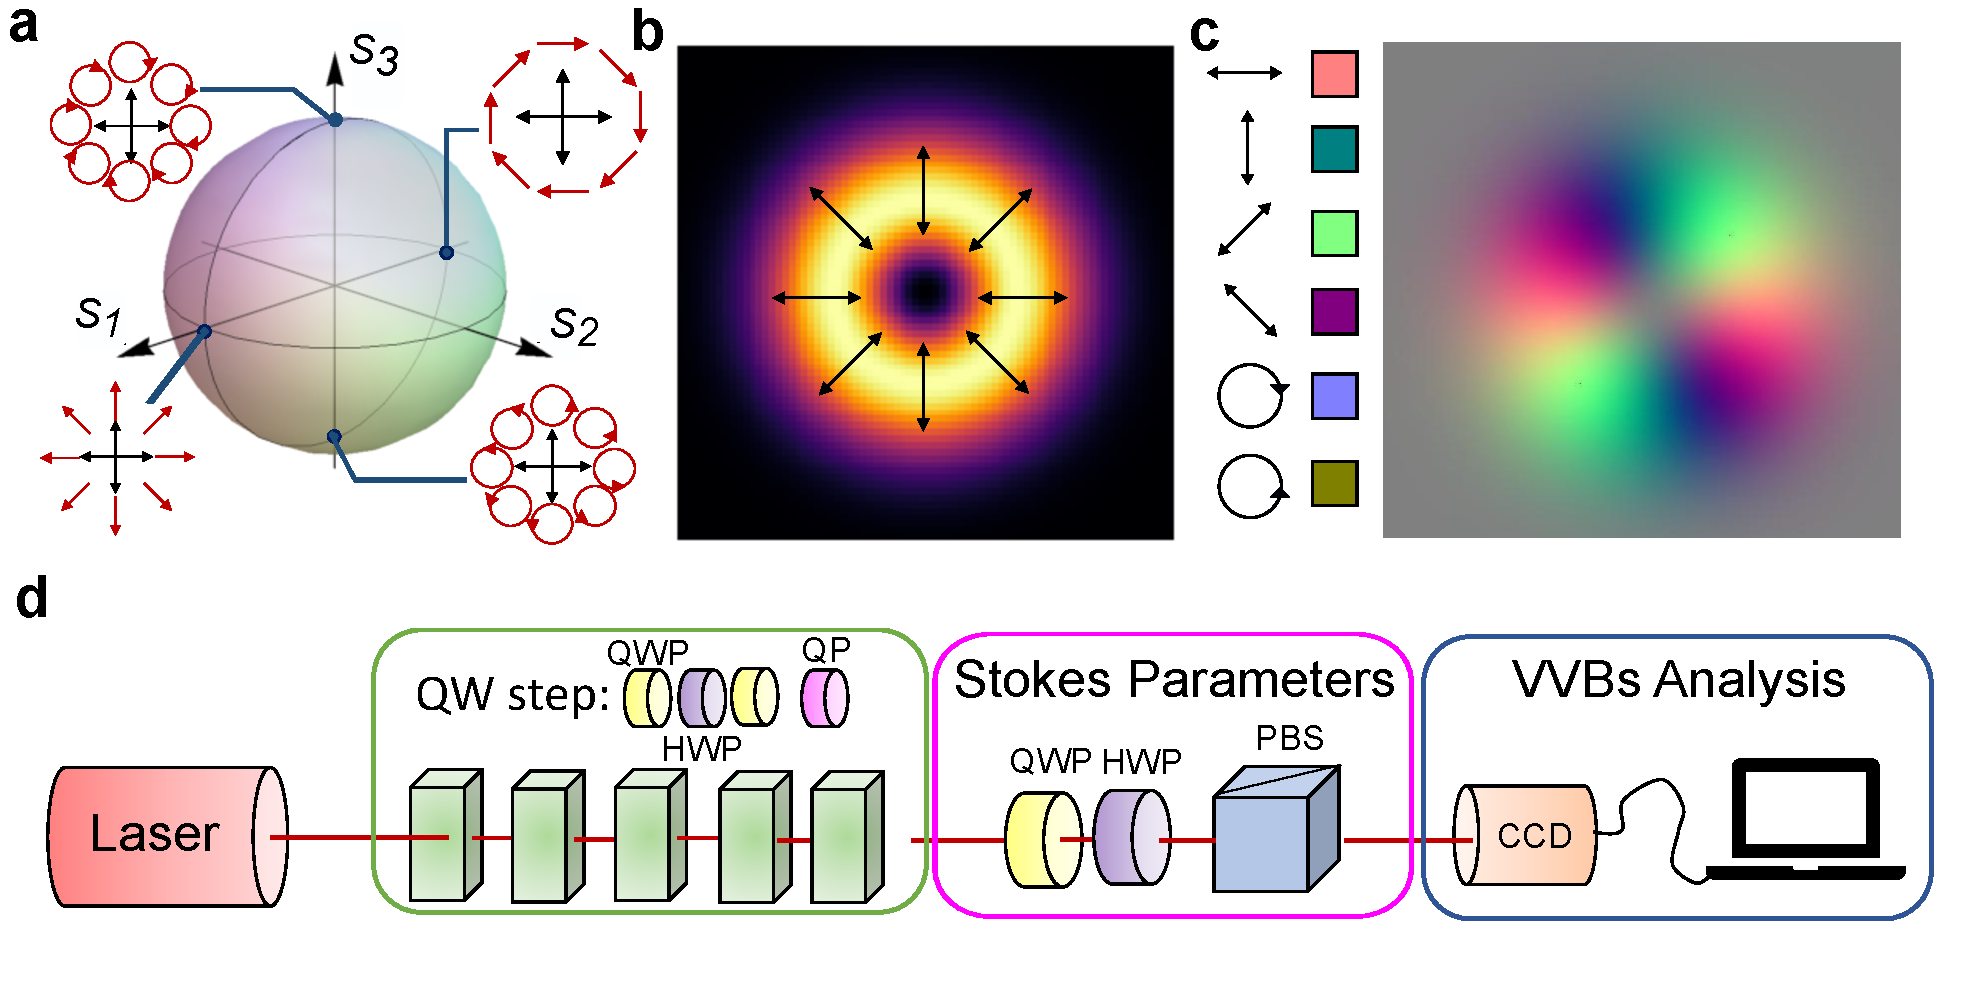
\includegraphics[width=0.8\textwidth]{VVBs-Fig1.pdf}
    \caption{
    	\textbf{(a)} High-order Poincar\'e sphere representation for $|m_{1,2}|=1$. Each point on the sphere surface corresponds to specific polarisation patterns. 
	    \textbf{(b)} A radially polarized \ac{VVB}: at a given point in the trasversal plane the polarisation vector has a different orientation. The Stokes parameters vary accordingly in the plane.
	    \textbf{(c)} Colour encoding of the polarisation pattern. 
	    The legend reports the correspondence between colours and the various polarisations.
	    On the right we have the resulting colour pattern for the VVB in panel {\bf b}.
	    Grey colour corresponds to unpolarised light.
	    \textbf{(d)} Experimental apparatus for the generation of \acp{VVB}. A continuous-wave laser emits a Gaussian beam ${\rm TEM}_{00}$ at $808$ nm. Light undergoes a 5-step quantum walk realized through a sequence of waveplates and q-plates.
    	A CCD camera-based detection stage acquires information on the Stokes parameters and the polarisation pattern. Based on the intensity measured at each pixels of the  camera, Stokes parameters are evaluated and converted into RGB-coloured pictures.
    }%
    \label{fig:VVBs:poinc_sphere}
\end{figure}


\section{Intro to OAM states}


\section{Experimental generation of Vector Vortex Beams}

\ac{OAM}-endowed states of light can be described using \ac{LG} modes.
These are solutions of the Helmholtz equation in the paraxial approximation, indexed by two integer numbers $(m, p)$, the former describing the azimuthal phase structure of the beam, and the latter describing its radial intensity profile.
Each~\ac{LG} mode carries a set amount of angular momentum, which in the single-photon regime equals $\hbar m$~\cite{allen1992orbital}.
\acp{VVB} can be obtained by superposing orthogonal polarisations to LG modes~\cite{padgett2004lights}.
More specifically, the electric field $\Vec{E}_{m_1m_2p}$ of a \ac{VVB} decomposes as the sum of two~\ac{LG} modes with same $p$ and different azimuthal numbers $m_1>m_2$ carried by orthogonal polarisations:
$\Vec{E}_{m_1m_2p}=\Vec{e}_L \cos{ \frac{\theta}{2}}\text{ LG$_{m_1p}$} +\Vec{e}_R e^{i \phi} \sin{ \frac{\theta}{2}}\text{ LG$_{m_2p}$}$,
where $\theta\in[0,\pi], \phi\in[0,2\pi]$ and the unit vectors $\Vec{e}_{L,R}$ stand for left and right circular polarisation, respectively.
For the purpose of this work we can ignore the radial number, setting $p=0$.
For any given value of the parameters $(m_1$, $m_2, \theta, \phi)$, the polarisation pattern of a \ac{VVB} can be mapped onto a generalized Poincar\'e sphere (cf. \cref{fig:VVBs:poinc_sphere}). In particular, we use the higher-order Poincar\'e representation in which the poles represent eigenstates of the total angular momentum but with opposite signs~\cite{milione2011higherorder}.
These polarisation patterns are reconstructed via the \emph{Stokes parameters} $S_{j}~(j=1,2,3)$, obtained by
measuring the output intensities $I_{b_j,1},I_{b_j,2}$ associated to a given choice of polarisation basis $\{b_j \}=\{b_1=( H,V )$, $b_2=( D,A )$, $b_3=( L,R )\}$ as $S_{b_j}=(I_{b_j,1}-I_{b_j,2})/(I_{b_j,1}+I_{b_j,2})$. %%
%This is a way to characterise a state via its \emph{Stokes parameters} at every point of the transverse %profile.
%To do this, we first measure the output intensities $I_{b_j,1},I_{b_j,2}$ associated to a given choice of %polarisation basis $b_j$, and then compute the value of the corresponding Stokes parameter $S_{b_j}$ as %$S_{b_j}=(I_{b_j,1}-I_{b_j,2})/(I_{b_j,1}+I_{b_j,2})$.
%The canonical choice for the polarisation bases is $b_1=(H,V), b_2=(D,A)$ and $b_3=(L,R)$.
%%
For a VVB, the values of $S_j$ depend on the coordinates in the transverse propagation plane {\cite{cardano2012polarization}}.
To visualize the polarisation patterns of \acp{VVB}, we use an RGB colour encoding in which the values of $S_j$ are interpreted as strengths of the corresponding colour. In Fig.~\ref{fig:VVBs:poinc_sphere}{\bf b} and {\bf c} we report an example of such colour-map for radially polarized \acp{VVB}.
A natural way to generate~\acp{VVB} is using \emph{q-plates}~\cite{marrucci2006optical,cardano2012polarization}, which are inhomogenous birefringent plates modifying the OAM of the incoming light conditionally to its polarisation. 
%~\cite{marrucci2006optical,cardano2012polarization}. 
In our scheme, \acp{VVB} are generated via a sequence of polarisation-controlling waveplates interspersing 5 cascaded q-plates (cf. Fig.~\ref{fig:VVBs:poinc_sphere}{\bf d}).
The apparatus implements a discrete-time QW in the angular momentum, where the order of LG modes takes the role of the \emph{walker} and it is changed according to the polarisation state, which embodies the \emph{coin} degree of freedom~\cite{zhang2010implementation,goyal2013implementing,cardano2015quantum,innocenti2017quantum,giordani2019experimental}.
%This apparatus implements a discrete-time QW in the OAM and polarisation degrees of freedom, in which the order of each LG mode takes the role of the \emph{walker}, and the polarisation that of the \emph{coin} degree of freedom
This allows to generate several classes of VVBs with OAM quantum numbers taking odd values in the interval $\{-5,..,5\}$.
We then collect images associated with different \acp{VVB} and use them to train and benchmark our ML-based approaches to classification , as discussed in the next sections.

\subsection{More stuff from SM}

The experimental platform, based on \ac{QW} in \ac{OAM} and polarisation degree of freedom \cite{innocenti2017quantum,giordani2019experimental}, is made up by $5$ q-plates (QPs) in cascade that can be interspaced by either half-waveplates (HWP) or quarter-waveplates (QWP). 
The action of the QPs on the joint OAM-polarisation states can be summarized as 
\begin{align}
  \Vec{e}_L \text{ LG}_m &\stackrel{\text{QP}}{\longrightarrow} \Vec{e}_R\text{ LG}_{m+2q} \notag\\ \Vec{e}_R \text{ LG}_m &\stackrel{\text{QP}}{\longrightarrow} \Vec{e}_L\text{ LG}_{m-2q}
\end{align}
where $q=1/2$. The HWPs compensate the polarisation flip operated by the QPs for the generation of higher order \ac{LG} modes. Conversely, the QWP acts on circular polarisations as an Hadamard transformation. Combining different sets of these waveplates inserted between consecutive QPs, we can generate \acp{VVB} with different pairs $(m_1,m_2)$ of OAM quantum numbers, and parameters $(\theta, \phi)$.
%sof the higher the increases the \ac{OAM} values associated to a \ac{VVB}. Moreover, using quarter waveplates it is possible to generate \acp{VVB} characterized by Laguerre Gauss modes with different azimuthal numbers $m_{1}>m_{2}$.


The experimental images are collected using a \ac{CCD} with a resolution of $1360 \times 1024$. 
However, we note that a resolution of $128 \times 128$ is already sufficient for the classification tasks we consider. Indeed, the training stage of the algorithms can be significantly speeds up by coarse-graining the images via an integration of its sub-blocks without any loss of information. 

For each generated \ac{VVB}, we measure the transverse intensity profile corresponding to each of the two outputs associated with each one of the three independent polarisation bases: $b_1=(H,V), b_2=(D,R)$, and $b_3=(L,R)$, where $\ket L\equiv \frac{1}{\sqrt2}(\ket H + \ket V)$, $\ket R\equiv \frac{1}{\sqrt2}(\ket H - \ket V), \ket D\equiv \frac{1}{\sqrt2}(\ket H + i \ket V), \ket R\equiv \frac{1}{\sqrt2}(\ket H - i \ket V)$.
This amounts, for each generated \ac{VVB}, to acquiring six intensities for each pixel of the \ac{CCD}. This representation is however redundant, as the properties of the VVBs only depend on the relation between the two intensities in each polarisation basis (which, in the single-photon regime, would correspond to the two outcome probabilities).
We therefore represent states using the \emph{higher-order Poincar\'e representation} \cite{milione2011higherorder,cardano2012polarization}. In this representation, each state is mapped into its three \emph{Stokes numbers} $S_{b_j}$, which equal the difference between the two intensities in each choice of polarisation basis:
\begin{equation}
  S_{b_j} = \frac{I_{b_j,1} - I_{b_j,2}}{I_{b_j,1} + I_{b_j,2}},
\end{equation}
where $b_j$ is one of the three canonical polarisation bases, and $I_{b_j,1}, I_{b_j,2}$ are the intensities corresponding to the two possible outcomes when measuring in the basis $b_j$.
In this representation, we therefore associate three real numbers to each each pixel in the \ac{CCD} camera. This means that each detected state is characterised by $128\times128\times3$ real numbers. To visualise these states, we represent the three Stokes numbers $S_{b_j}$ using an RGB colour encoding. In particular, the strengths of the colours red, green and blue are associated with the $S_{1}$, $S_{2}$ and $S_{3}$ parameters,  respectively.
This allows us to map each VVB state into a three-channel coloured image.

For the purpose of the classification algorithms described in~\cref{sec:VVBs:classification,sec:VVBs:dimensionality_reduction,sec:SVMs}, each state is represented as a real vector of length $128\times128\times 3$.


\begin{figure}[tb]
	\centering
	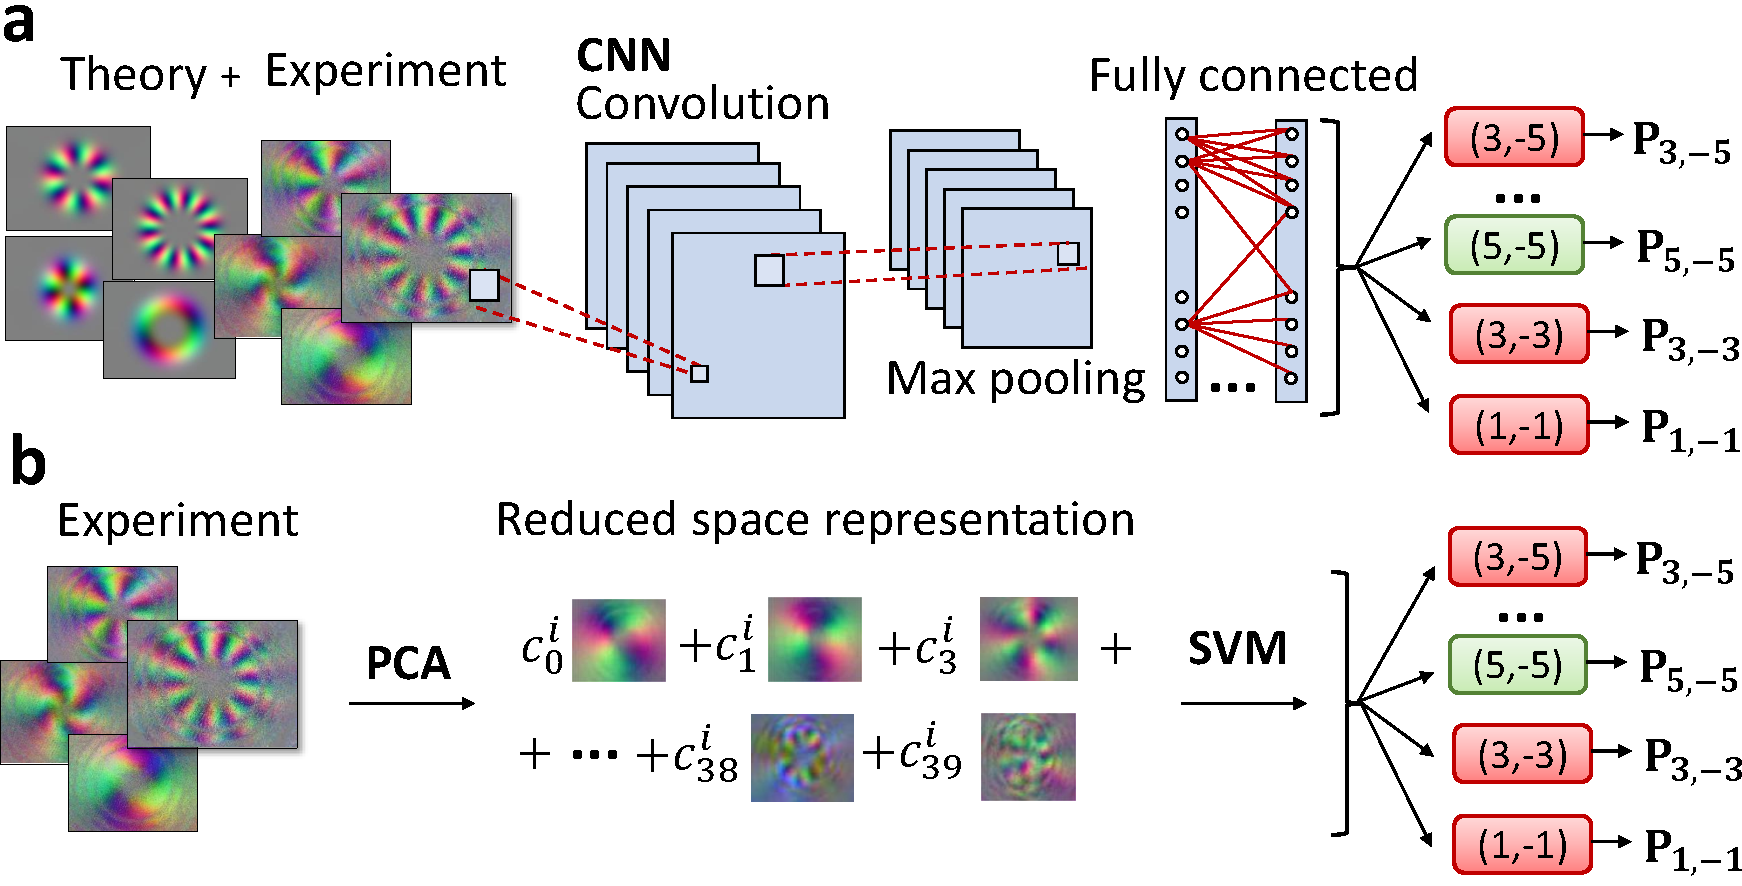
\includegraphics[width=\textwidth]{conc_VVB_2.pdf}
	\caption{
	\textbf{(a)}
	Working principles of \acp{CNN}. The training set consists of a series of simulated images, plus some others collected from the experimental platform.
	\textbf{(b)}
	Classification scheme using linear \ac{PCA}.
	After reducing the dimensionality of the dataset via \ac{PCA}, a linear \ac{SVM} is used to classify experimental images. 
	}
	\label{fig:VVBs:class_techniques}
\end{figure}

\begin{figure}[tb]
    \centering
    \includegraphics[width=0.8\textwidth]{VVBs-Fig3.pdf}
    \caption{
	    \textbf{(a)} Comparison between expected and recorded polarisation patterns for some \acp{VVB} of the ensemble in table, with the corresponding values $(m_1,m_2)$.
	    \textbf{(b)} Scaling of the average accuracy per class when classifying states into one of the $15$ VVB classes,
	    against the fraction of experimental images in the training set. 
	    Inset: best truth table.
	    Rows (columns) stand for the possible $(m_1,m_2)$ pairs (as assigned by the CNN). The matrix elements have been averaged over $100$ experimental images per class.
    }%
    \label{fig:VVBs:resultsCNN}
\end{figure}



\section{Classification of VVBs}
\label{sec:VVBs:classification}


\subsection{CNNs}
\label{sec:VVBs:CNNs}

\subsubsection{From main}

We show here how to train a \ac{CNN}  to retrieve the  parameters $(m_1,m_2)$ characterizing a given VVB  from experimentally  measured Stokes parameters .
\acp{CNN}  are translation-invariant deep NNs well-suited for image classification~\cite{lecun2015deep},  to recognize off-center images and segmented handwritten digits~\cite{simard2003best,ciresan2011flexible},
and for facial recognition tasks~\cite{matsugu2003subject}. 
In their simplest form, \acp{CNN} work by first applying a \emph{convolutional layer}, which consists of a series of nonlinear transformations applied to the input images, followed by a \emph{max-pooling layer}, which downsamples and filters the information extracted by the previous layer. Finally, a fully connected layer functions as a \emph{classifier}, categorizing the information extracted in the previous layers into one of a small number of possible output categories
 (cf. \cite{SI}).
 
The network is first fed with a training set made out of simulated images of \acp{VVB} achievable with a five-step \ac{QW}.
The task is then to discern between $15$ classes, corresponding to the pairs $(m_1,m_2)$ in Fig.~\ref{fig:VVBs:resultsCNN}\textbf{a}.
For each class we generate states with $\theta=\pi/2$ and $\phi\in[0,2\pi]$. The size of the training set is $400$ images per class. Additional $100$ simulated images per class are used to benchmark the performance during training. In these conditions, the network achieves an accuracy of $100\%$ . 
We then collect $100$ experimental images per class, to use as new validation set (cf. Fig.~\ref{fig:VVBs:class_techniques}{\bf a}). Fig.~\ref{fig:VVBs:resultsCNN}{\bf a}-{\bf b} shows the mean accuracy per class against the fraction of experimental images gradually inserted in the training set, starting from one consisting of computer-generated images only.
Remarkably, a small increase of the number of experimental images in the training set results in a good accuracy reached by the network (cf. Fig.~\ref{fig:VVBs:resultsCNN}{\bf b}): an average accuracy of $\sim 0.989$ is already obtained when $12.5\%$ of the training set is composed of experimental images.
%, as reported in Fig.~\ref{fig:VVBs:resultsCNN}c. 



We use a similar approach to retrieve the position on the Poincar\'e sphere corresponding to states generated with fixed $(m_1,m_2)$.
We then test the performance of the CNN in the classification of each recorded VVB according to the values $(\theta,\phi)$ for $m_2=-m_1=1$ .
To  achieve this, the network should discriminate rotations in the polarisation patterns (i.e. changes in $\phi$) and variations in the colour tone (i.e. changes in $\theta$).  A drawback of using  any type of classifier for this task is that VVBs with $|m_i|\gg1$ display a polarisation pattern whose periodicity decreases as $\frac{2\pi}{|m_1-m_2|}$ (cf. Fig.~\mbox{\ref{fig:VVBs:resultsCNN}}{\bf a})~\cite{fickler2012quantum,dambrosio2013photonic}.
This complicates the recognition of $\phi$, as changes in the phase generate only small rotations of the pattern.
Furthermore, the classification of the VVB on the sphere requires a discretization of  $\theta$ and $\phi$, which results in dividing the sphere in sectors. This means that VVBs placed at the borders of these intervals are more difficult to assign to a specific class.
The network is then trained with  simulated images  corresponding to different positions on the sphere. 
%(that is, different values of $(\theta,\phi)$).
The latter is divided in 26 sectors as follows: $\theta$ is divided in $3$ intervals $\left[k \frac{\pi}{8}, (k+2) \frac{\pi}{8}\right]$ ($k=2n+1$,  $n \in \{0,1,2\}$), while $\phi$ is split in the 8 classes $\left[t \frac{\pi}{4}, (t+1) \frac{\pi}{4}\right]$ with $t \in \{0,...,7\} $. The remaining two classes, representing the two poles, correspond to $\theta \in \left[0, \frac{\pi}{8}\right]$ and $ \left[ \frac{7}{8} \pi, \pi\right]$, with no distinction in $\phi$ [cf. Fig. \ref{fig:VVBs:PCAresults}{\bf a}].
We  generate $500$ images per class in the training set, and $125$ per class  for the  validation one. The maximum accuracy  achieved is $\sim 0.90$. This result, which is inferior with respect to what is achieved by only inferring $m_{1,2}$,  confirms the sub-optimality of the method when we had to artificially coarse-grain two continuous parameters.  
%when an artificial binning of continuous parameters into discrete classes, which then necessarily leads to poor prediction accuracies for values close to the boundaries of the classes.

%To achieve this, the network must be able to discriminate patterns only differing by a rotation (corresponding to changes of $\phi$), as well as by variations in the colour tone (corresponding to different values of $\theta$).
%To implement this as a classification task, we fix $m_1=-m_2=1$ and discretize the possible values of $\theta,\phi$ into $26$ distinct classes.
%These classes are defined by partitioning the spherical coordinates as follows: $\theta$ is subdivided into the five classes $[0,\pi/8], [\pi/8, 3\pi/8], [3\pi/8, 5\pi/8], [5\pi/8, 7\pi/8], [7\pi/8, \pi]$. Each one of these classes, except for the two surrounding the poles, is then subdivided into $8$ different sectors, each one corresponding to values of $\phi$ belonging to a different interval of the form $[k\pi/4,(k+1)\pi/4]$ with $k\in\mathbb N$ (see also Fig.~\ref{fig:VVBs:PCAresults}a).
%%The network is then trained with simulated images corresponding to different positions on the sphere (that is, different values of $(\theta,\phi)$).
%%We use $500$ images per class in the training set, and $125$ per class in the test set. The maximum accuracy achieved is $\sim 0.90$. The main reason for the suboptimality of this result is that this method involves an artificial binning of continuous parameters into discrete classes, which then necessarily leads to poor prediction accuracies for values close to the boundaries of the classes.

\subsubsection{From SM}
We describe here in more detail the structure of the \ac{CNN} used to classify the experimental images.
In a standard \ac{CNN}, the convolution in a particular location $(x,y)$ is obtained by computing the inner product between a $k \times k$ sub region of the input image and a filter of the same size. Repeating this process for each location on the input image, it is possible to obtain an activation map associated to specific features. Typically, more than one filter is used in one convolution layer and $N$ features are extracted.
A max-pooling layer is used immediately after the convolutional layer to reduce the number of parameters. The output of the previous layer are then divided into blocks of size $p \times p$, and the $\max$ function is applied over each block.
Finally, a fully connected layer classifiers the data by determining which features are most correlate to a particular class.
At the beginning, the filters of the features extractors are randomly initialized. Consequently, they are computed via a back-propagation process to optimize the classification of a training set.

To build and train the \ac{CNN} we used the Python library \emph{Keras}~\cite{chollet2015keras}.
We used a CNN with three feature extractors and one classifier. In each convolution layer we apply $32$ filters of size $3 \times 3 \times 3$ and as activation function is used the Rectified Linear Unit (ReLU). Subsequently, the max function is applied over blocks of size $2 \times 2 \times 3$  in max-pooling layers. %\redComm{(unclear)}. 
The final classification is performed by a fully connected layer which uses a sigmoid activation function. The network training consists of a finite number of epochs each of which composed of $200$ training steps and $100$ validation steps. 


\subsection{Dimensionality reduction}
\label{sec:VVBs:dimensionality_reduction}

\subsubsection{From main}

We now present an alternative approach to classify \acp{VVB} from experimental data, leveraging \ac{DR}.
Such algorithms are typically used to obtain efficient representations of large datasets~\cite{cunningham2008dimension,fodor2002survey}.

This has several advantages, from easing data visualisation, to improving the efficiency of classification and regression algorithms, which can be used on the reduced representation of the data.
In particular, we employ a linear 
\ac{PCA} algorithm, which works by representing each datapoint as a vector in some high-dimensional space $\RR^n$, and finding the directions in such space that capture the maximum amount of information about the dataset~\cite{jolliffe2011principal,jolliffe2016principal}.
The rationale for using \ac{PCA} in this context is that, although experimental images live in extremely high-dimensional spaces (whose dimension is of the order of the number of pixels in the \ac{CCD} camera), the underlying dimension of the generated \acp{VVB} is typically much lower.
This means that, although the experimental dataset will \emph{a priori} seem like a complicated bundle of high-dimensional vectors, the underlying data is actually characterizable by a small number of parameters. Furthermore, the linearity of the mapping preserves the convexity of the VVB space and thus its geometrical structure. We then expect that the new description for expressing the experimental images in the reduced space provides a synthetic description for capturing the features of VVBs encoded in the measurements (the intensities in three polarisation bases $\{b_j\}$, cf. \mbox{\cite{SI}}).

This resembles a form of \emph{unsupervised} learning, as we gain useful information about the origin of the images are inferred without feeding the algorithm with any knowledge of the underlying process.
 
\begin{figure}[t]
    \centering
    \includegraphics[width=0.8\linewidth]{VVBs-Fig4.pdf}
    \caption{
		\textbf{(a)} High order Poincar\'e sphere for \acp{VVB} with $|m_{1,2}|=1$. Magenta-coloured parallels (Blue-coloured meridians) mark intervals between consecutive values of $\theta$ ($\phi$). 
		Along a meridian the colours of the pattern vary from the hottest to the coldest one. Along a parallel, the patterns rotate. 
		\textbf{(b)}
		Comparison between experimental and simulated \ac{VVB} images for different angles $(\theta, \phi)$.
		\textbf{(c)}
		Distribution of fidelities obtained comparing each experimental VVBs with its reduced 3D representations given by PCA. Projecting each image onto its first three principal axes and rescaling brings the data (orange points) onto a sphere in 3D, as shown in the inset. The inner (outer) black (semi-transparent) sphere is added for contrast [radius equal to that of the point with smaller (larger) radius].
		\textbf{(d)}
		Average prediction accuracy of a linear \ac{SVM} classifier, trained and tested after applying linear DR to the data, against the number of reduced dimensions $n_c$.
		For each of the 15 classes (cf.~\cref{fig:VVBs:resultsCNN}a) in which the experimental dataset was divided, we show in the inset the true-table. 
    }%
    \label{fig:VVBs:PCAresults}
\end{figure}


As a notable example, we apply these observations to \acp{VVB} with $m_2=-m_1=1$, which can be pictured as lying on a sphere, in the higher-order Poincar\'e representation. 
%of the form $c_0 \ket{L,m=1} + c_1 \ket{R, m=-1}$ with $\abs{c_0}^2+|c_1|^2=1$.
%The inclusion of only two orthogonal basis states makes these states effectively equivalent to a single qubit. 

%Knowing that a single qubit can be represented with a Bloch sphere we can expect, as per our previous argument, that the corresponding experimental images will also arrange on a sphere embedded in the high-dimensional space.
Indeed, \ac{PCA} applied to the experimental dataset of Fig. \ref{fig:VVBs:PCAresults}{\bf b}, 
reveals that only three directions capture most of the information content of the images. Projecting the images along these three principal components, we recover that the data is arranged in the form of a three-dimensional sphere embedded in the high-dimensional space of experimental [cf. inset of~\cref{fig:VVBs:PCAresults}{\bf c}].
Remarkably, this was not obvious from the experimental dataset alone, but was easily found via \ac{DR}. This result highlights the potential of {\ac{DR}} to  reveal features of the underlying states generating a given experimental dataset, also in the presence of experimental noisy conditions (cf.~\cite{SI}).


To assess the accuracy of such reconstruction, we compute the average fidelity $\mathcal F_{\text{avg}}$ between the expected state and the one found by our analysis with PCA . As shown in the histogram of Fig.~\ref{fig:VVBs:PCAresults}c,  this is found to be $\mathcal F_{\text{avg}}\sim0.96$ (standard deviation $\sim0.01$), thus certifying the quality of the reconstruction.

\subsubsection{From SM}

We discuss here our application of \emph{dimensionality reduction} to characterize experimental images. The main idea behind dimensionality reduction algorithms is to reduce the dimensionality of a dataset while retaining as much of its important features as possible. More specifically, we use linear \ac{PCA}~\cite{jolliffe2016principal}. The goal of this dimensionality reduction algorithm is to find the directions upon which projecting the dataset vectors gives the maximum amount of variance. More specifically, if the dataset is comprised of $N$ (real) vectors of length $M$, defining the \emph{data matrix} $\bs X$ as the $N\times M$ matrix whose $i$-th row is the $i$-th dataset vector, \ac{PCA} consists in finding the vectors $\bs a\in\RR^{M}$ that maximise the variance of $\bs X\bs a$. This turns out to be equivalent to diagonalising $\bs S\equiv \tilde{\bs X}^T\tilde{\bs X}/(N-1)$, where $\tilde{\bs X}$ is the \emph{centered data matrix}, which is equal to $\bs X$ modulo each of its columns shifted in order to average to zero.
The first $k$ \emph{principal components} found by \ac{PCA} are then the $k$ eigenvectors of $\bs S$ corresponding to the largest $k$ eigenvalues.
Note that these principal components are themselves vectors of the same ``type'' as the data vectors. This means that \ac{PCA} effectively generates a set of data vectors which ``optimally represent'' the information content of the given dataset.

For example, in our case, each row of $\bs X$ is a vector of length $128\times128\times3$ containing the Stokes parameters $S_{b_1}, S_{b_2}, S_{b_3}$ for each pixel of the camera.
Because each image corresponds to such a vector, and vice versa each such vector corresponds to the image of a \ac{VVB}, we can represent the principal components found by \ac{PCA} again in the form of images, which allows us to gain some intuition into the type of principal components that optimally represent the data according to \ac{PCA}.

Let now $\rho$ be the density matrix characterizing a \ac{VVB} state. The corresponding image can be associated to the set of real numbers $p_k=(\mathcal U\rho\mathcal U^\dagger)_{kk}$ with $\mathcal U$ the unitary operator that performs the basis change from the \ac{OAM} to the position basis. In other words, $\rho$ describes the state in the OAM-polarisation basis, which is the basis in which the generated states are efficiently described, whereas $\mathcal U\rho\mathcal U^\dagger$ describes the same state in the position basis, which is the one in which the CCD camera operates on.
The set of detected probabilities is then given by~\footnote{It should be noted that, while here we use a formalism and vocabulary evocative of quantum states, the states actually used in the experiment are classical. This in now way impacts the formal description of the protocol, and the only thing that should change when the states used are classical is that the probabilities $\bs p$ should be reinterpreted as intensities.}
$\bs p=\on{diag}(\mathcal U\rho\mathcal U^\dagger)\equiv\Psi(\rho)$,
where $\Psi$ is defined as the linear map that sends $\rho$ to the set of measured probabilities $\bs p$.
Crucially, the linearity of $\Psi$ implies that it preserves the \emph{convexity} of the space of states, and therefore many of its geometrical features.
For example, if we consider the set of states of the form $c_0 \ket{\uparrow,m=m_1} + c_1 \ket{\downarrow,m=m_2}$ with $m_1\neq m_2$, then the associated density matrices will be arranged to form a three-dimensional sphere embedded in the full state space (because these are effectively different states of a single qubit).
Thanks to the linearity of $\Psi$, \emph{the corresponding probabilities $\bs p$ will also be contained in a spherical surface}, up to possible rescaling of the axes.
In other words, the Bloch sphere of the original two-dimensional system is still present, albeit hidden, in the experimental images, embedded into an extremely high-dimensional space.

\begin{figure*}[tb]
  \centering
  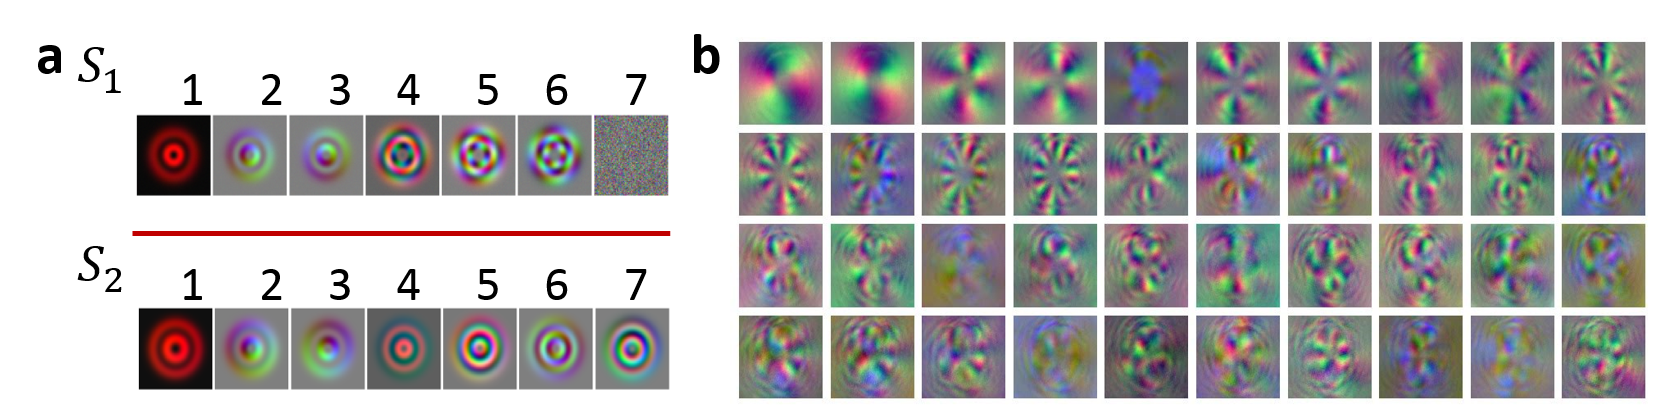
\includegraphics[width=0.98\textwidth]{S1_fig.png}
  \caption{
      \textbf{a,}
       Principal components obtained using PCA on simulated datasets of noisy VVB. The first (second) row shows the first seven principal components obtained on the dataset $\mathcal S_1$ ($\mathcal S_2$). 
       The first 6 (all 7) components correspond to non-vanishing singular values.
       \textbf{b,} First 40 principal components individuated in the experimental dataset corresponding to the 15 classes labelled by $(m_1,m_2)$, discussed in the main text.%
    }
    \label{fig:S1}
\end{figure*}

To see the usefulness of these ideas to understand the type of states generated by a given apparatus, we consider here two examples of applications of \ac{PCA} for different types of input states. 
In all of these cases, \ac{PCA} is applied without any previous knowledge of the type of states that underly the observed experimental images, and is therefore to be considered a type of \emph{unsupervised learning}.
Consider a simulated set of images corresponding to VVBs of the form
$c_1\ket{L,m=1}+c_2\ket{R,m=2}$ and
$c_1\ket{L,m=1}+c_2\ket{R,m=4}$, where the coefficients $c_i$ are sampled uniformly at random from the set of $c_{1},c_2\in\mathbb{C}$  such that $|c_1|^2+|c_2|^2=1$ (\emph{i.e.} uniformly sampled on the Bloch sphere).
Applying PCA to this dataset, we find six non-vanishing singular values, whose associated principal components are given in Fig.~\ref{fig:S1}a.
This is consistent with the dimension of the subspace  spanned by states of the form $\mathcal S_1=\{c_1\ket{L,1}+c_2\ket{R,2}, c_3\ket{L,1}+c_4\ket{R,4}\}$,  as the set of corresponding density matrices is spanned by the six orthogonal matrices
$X^{(1,2)}, X^{(1,4)}, Y^{(1,2)},Y^{(1,4)},Z^{(1,2)}\pm Z^{(1,4)}$, where $X^{(i,j)}=\ketbra{i}{j}+\ketbra{j}{i}$ is the Pauli $X$ matrix acting on the $(i,j)$ subspace, and similarly for $Y^{(i,j)}$ and $Z^{(i,j)}$.
On the other hand, if the dataset under consideration consists of states of the form $\mathcal S_2=\{c_1\ket{L,1}+c_2\ket{R,2}, c_3\ket{L,3}+c_4\ket{R,4}\}$, then \ac{PCA} finds \emph{seven} principal components associated with non-vanishing singular values (see Fig.~\ref{fig:S1}a).
This is consistent with the underlying state space being spanned by the seven orthogonal Hermitians:
\begin{equation}
\begin{gathered}
    X^{(1,2)}, \,\, X^{(3,4)}, \,\,
    Y^{(1,2)}, \,\, Y^{(3,4)}, \\
    Z^{(1,2)},\quad
    -Z^{(1,2)} + 2 Z^{(1,3)}, \\
    -Z^{(1,2)} - Z^{(1,3)} + 3 Z^{(1,4)}.
\end{gathered}
\end{equation}
These matrices can be obtained by direct analysis of the type of states contained in $\mathcal S_2$ and then finding a set of orthogonal Hermitian matrices generating the corresponding set of density matrices.
It is worth noting how this method provides a quick and easy way to gain useful information about the dimensionality of generated states, as well as about other properties such as specific symmetries, which, as shown in~\cref{fig:S1}, are often picked up by the principal components.


\subsection{Support vector machines}
\label{sec:SVMs}

\subsubsection{From main}

We now show how the reduced representations provided by \ac{PCA} can function as starting point to train a classifier with accuracy comparable with the \ac{CNN}, whilst requiring a significantly reduced amount of computational resources.
%More precisely, we use as classifiers linear {\acp{SVM}}~\cite{hearst1998svm}. These supervised learning algorithms categorize data by finding the hyperplane that optimally separates the training dataset in accordance with the corresponding labels. 

As done for the \ac{CNN}, we consider the task of classifying experimental dataset of \ac{VVB} states, indexed by $(m_1,m_2)$ . We train the \ac{SVM} on the reduced space obtained via \ac{PCA}, applied to the experimental dataset reported in~\cref{fig:VVBs:resultsCNN}{\bf a}. This stage significantly improves the training cost of the classifier since the latter will work on a synthesized description of the high-dimensional space of images in which the features of each class can be easily recognized.
%This not only significantly speeds up training the classifier, but also makes for a more %robust classification, thanks to the property of dimensionality reduction algorithms to %weed out statistical and experimental noise.
%What's more, the geometrical picture offered by the reduced representation tells us when %we should expect this classification to be accurate: \ac{PCA} effectively retrieves the %description of the states in the generalized Bloch representation (cf.~\mbox{\cite{SI}}), %therefore the classification will give good results whenever the states are linearly %separated in state space.
%%\%rmv{We consider classes of the form $(m_1,m_2)$, as we did for the CNN.}
%When tested on the same dataset used previously for the {\acp{CNN}} %(cf. Fig~\ref{fig:VVBs:class_techniques}), the \ac{SVM} achieved an average %accuracy of $~98\%$ for the task of recognizing to which of the $15$ \ac{VVB} %classes $(m_1,m_2)$ a given state belongs to.
%Applying the method to our dataset , we get an average $\sim98\%$ accuracy after reducing the dimension of the data to 40 via linear \ac{PCA} [cf. \mbox{\cite{SI}}].
The~\ac{SVM} was trained on half of the experimental data, with the other half used to test the resulting accuracy. A breakdown of the classification performance is reported in the inset of~\cref{fig:VVBs:PCAresults}{\bf d}, where we detail how the images belonging to each class were classified.

We used here a \emph{linear} SVM, instead of a commonly used SVM with RBF kernel, because we found it to perform better: an RBF kernel was found to give, in our case, an average accuracy of only $\sim94\%$.
Furthermore, in~\cref{fig:VVBs:PCAresults}{\bf d} we highlight how the average overall accuracy depends on the dimension of the reduced representation: $\sim 25$ dimensions are already sufficient to get good average accuracies.

\subsubsection{From SM}

Once \ac{PCA} has been used to find reduced representations for the experimental images, simple classification methods such as \acp{SVM}~\cite{hearst1998support,shawe2000support} can be used to categorize them.
We use here in particular a \emph{linear}, multiclass \ac{SVM}, whose goal is to find hyperplanes in the feature space that optimally separate the datapoints corresponding to different classes.
During the training phase, a set of training experimental images is used to find the separating hyperplanes, which can then be used to classify new experimental images.

We train \ac{PCA} on the reduced representation found by extracting via \ac{PCA} the first $40$ principal components of the training dataset shown in Fig.~\ref{fig:S1}b. The goal is, similarly to what we did with the \ac{CNN}, to classify experimentally generated \acp{VVB} according to one of $15$ classes defined by their OAM parameters $(m_1,m_2)$.
% In our work a linear support vector machine (SVM) has been employed for this task. Support vector machines are very well-known linear classifiers in machine learning. The algorithm is fed with a series of labelled data during the training stage as to retrieve the optimal hyperplane which separates the elements of different classes. In the present case the SVM finds the optimal separation between experimental images of the training set expressed in the reduced space, described by the principal components in Fig. \ref{fig:S1}b.
The average classification accuracy achieved on images not included in the training set is $\sim 98 \%$. This result confirms that the description provided by \ac{PCA} is sufficient to capture the important features of the generated states, thus allowing for a dramatically more efficient classification scheme.


\section{Discussion}
\label{sec:VVBs:discussion}

We presented a new approach to classify \acp{VVB} leveraging ML techniques. We demonstrated how the use of inference strategies based on CNNs and PCA (enhanced by SVMs) allows to extract efficiently properties of high-dimensional photonic \ac{VVB} systems.
In particular, DR was used to obtain a deeper understanding of the underlying geometrical properties of the experimentally generated states, without requiring prior knowledge about the physics of the generation apparatus.
% this is not quite right
By embedding a variety of {\ac{ML}} algorithms into our experimental pipeline, the task of characterising structured light is made significantly broader in the methods, ranging from supervised to unsupervised learning, and more flexible in the applications, classification and regression tasks.
%
%Then, the investigation of different techniques in the ML field has provided a more general framework for the characterization of structured light. 
% 
While paving the way to further experimental validations -- potentially also in experimental settings that do not rely on optical networks -- we believe that numerous tasks of relevance to modern photonics could benefit from introducing similar {\ac{ML}} ideas into their characterization protocols. These techniques can prove to be useful add-on to tasks ranging from the design of automatized approaches to the characterization of experimental platforms and experiments, to the provision of solutions to OAM demultiplexing in the context of classical and quantum communication and, more generally, for the use of structured light in quantum technologies.

\textit{Note--} During the reviewing process of this manuscript, the authors
became aware of a related work~\cite{liu2019superhighresolution} addressing a similar topic.
